%%=============================================================================
%% Conclusie
%%=============================================================================
\chapter{Conclusie}%
\label{ch:conclusie}

Google Cloud Platform is zeker niet geschikt voor deze specifieke use-case, we moeten dus enkel nog Azure en AWS vergelijken.
Het is duidelijk dat Azure betere resultaten kan voorleggen voor deze use-case dan AWS, zowel de nauwkeurigheid als de gewogen nauwkeurigheid zijn voor alle data-sets hoger. Azure ondersteunt ook meerdere frameworks en biedt de mogelijkheid om modellen lokaal te exporteren. Ook de documentatie van Azure is veel uitgebreider dan die van AWS. Zowel AWS als Azure bieden tutorials aan om de mensen opweg te zetten, en in beide platformen is er een default dataset voorzien waar nieuwe gebruikers kunnen op experimenteren. 
\begin{figure}[h]
    \caption{Barchart die de nauwkeurigheden van AWS en Azure vergelijkt per percentage van de dataset dat werd gebruikt als trainingsdata.}
    \centering
    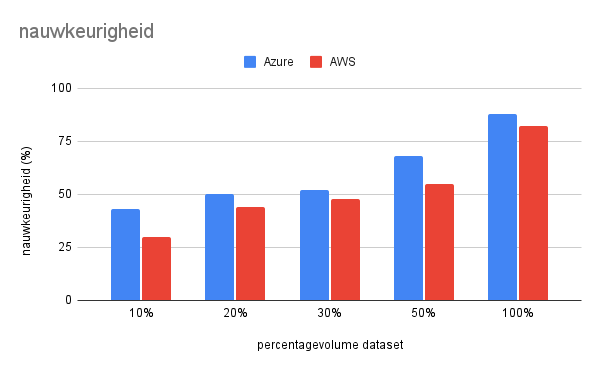
\includegraphics[width=0.5\textwidth]{nauwkeurigheid}
\end{figure}

\begin{figure}[h]
    \caption{Barchart die de gewogen nauwkeurigheden van AWS en Azure vergelijkt per percentage van de dataset dat werd gebruikt als trainingsdata.}
    \centering
    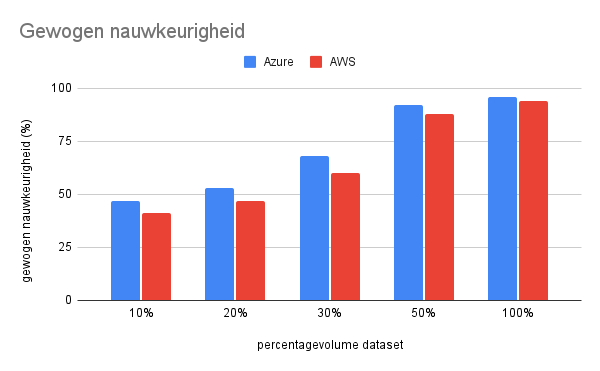
\includegraphics[width=0.5\textwidth]{Gewogen nauwkeurigheid}
\end{figure}


\section{toegevingen}
De modellen die in dit onderzoek worden gegenereert kunnen slechts 1 tag voorspellen, terwijl PIMLayers tag-systeem meerdere soorten tags ondersteunt. Dit wil zeggen dat er voor elke tag een ander model zou moeten worden gegenereerd, en dat ook nog eens voor elke klant. Het zou dan ook interessant kunnen zijn om de eindgebruiker te laten instellen voor welk type tags er een model moet worden voorzien en voor welke niet.

Het taxonomie systeem van PIMLayer ondersteunt ook meerdere tags per bestand, de modellen die voor dit onderzoek zijn gegenereerd konden hier moeilijk mee om, zo bleek in de zoektocht naar welke tag de modellen zouden moeten gaan voorspellen. 

\section{verder onderzoek}
Nu er een keuze kan gemaakt worden qua provider is de volgende uitdaging om deze te integreren in PIMLayer zelf. Er moet ook nog nagedacht worden over hoe en op welke manier dit zou moeten gebeuren: moeten alle tags worden voorspeld? wat met meerdere tags per bestand?...

% TODO: Trek een duidelijke conclusie, in de vorm van een antwoord op de
% onderzoeksvra(a)g(en). Wat was jouw bijdrage aan het onderzoeksdomein en
% hoe biedt dit meerwaarde aan het vakgebied/doelgroep? 
% Reflecteer kritisch over het resultaat. In Engelse teksten wordt deze sectie
% ``Discussion'' genoemd. Had je deze uitkomst verwacht? Zijn er zaken die nog
% niet duidelijk zijn?
% Heeft het onderzoek geleid tot nieuwe vragen die uitnodigen tot verder 
%onderzoek?



